\subsection{Value functions in belief wealth space}\label{ssec:val-func}

First, we look at value functions found by using different utility functions in~\autoref{fig:val-func}.
As described in~\autoref{sec:methods} augmented state space encodes the wealth and the belief of the agent. 
Additionally, in our case, time can be related to wealth by the simple formula:

\begin{align*}
\text{time} = \frac{\text{wealth}}{\text{observation\ cost}}
\end{align*}

The policy is the action with maximum return for each belief wealth pair, which is the line that separates the blue (waiting) and the orange (selling) area in~\autoref{fig:val-func}. For example, in the very first plot, the agent always sells at 0.8 belief for any wealth value. We call this line the belief threshold.

\begin{figure}[h]
    \centering
    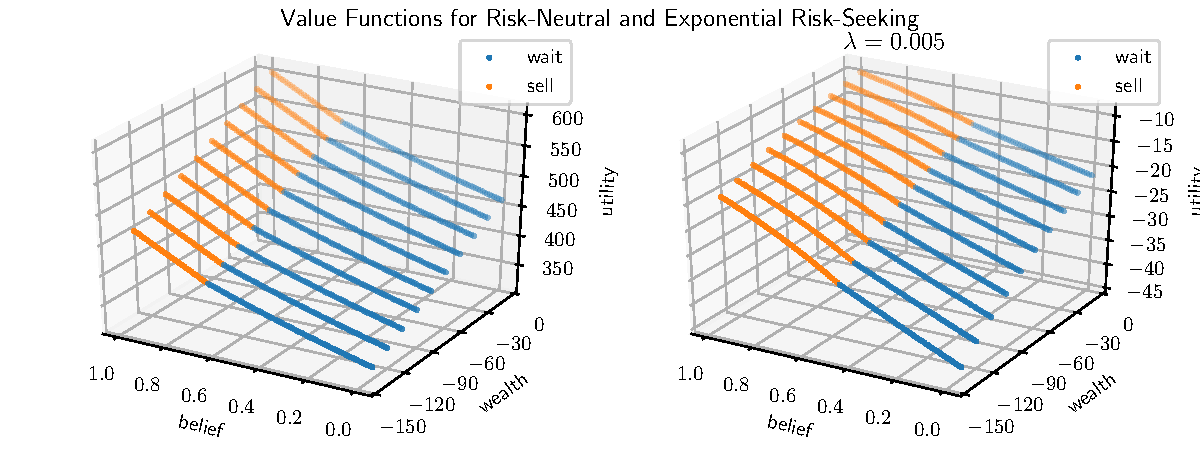
\includegraphics[width=0.99\linewidth]{img/exp_policy.pdf}\\
    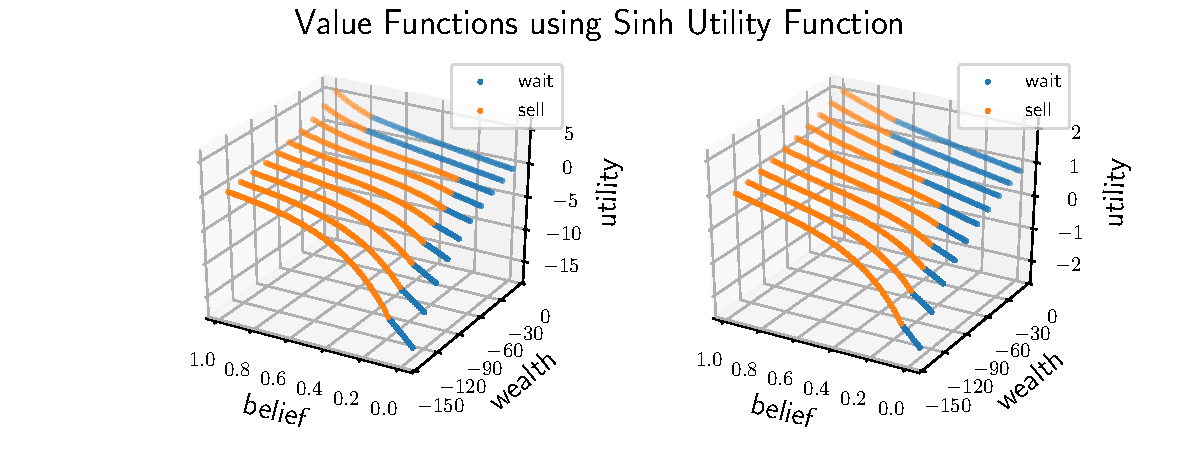
\includegraphics[width=0.99\linewidth]{img/sinh_policy.pdf}\\
    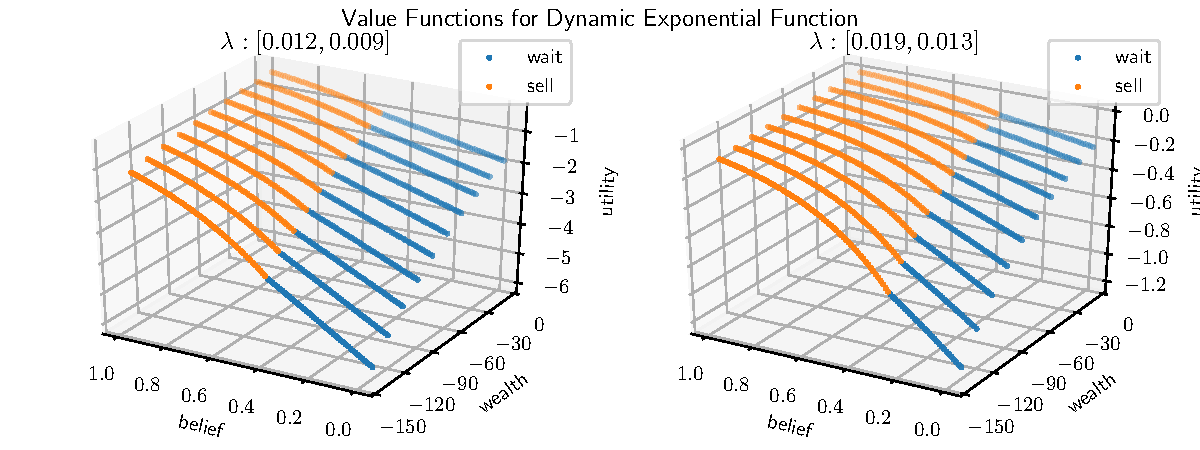
\includegraphics[width=0.99\linewidth]{img/dyn_policy.pdf}
    \caption{Value functions exhibiting different risk-behaviors; from top left: risk neutral agent (utility function is the identity function), risk-seeking agent with exponential utility function, two fixed time agents with different time thresholds, two agents with dynamic exponential utility function.}\label{fig:val-func}
\end{figure}


In the first row, we present value functions that are found by using the risk-neutral UF (identity function) and an exponential UF. Both functions result in agents simply selling above a certain belief threshold, regardless of the current wealth.
% TODO do we need a policy plot to make this clear?
Exponential UF sets this threshold with the $\lambda$ parameter, which is displayed above the plot.
A negative $\lambda$ induces risk-averse behavior, which results in selling with higher belief than the risk-neutral agent.

The second row shows policies derived by the $\text{sinh}$ UF. As oppesed to the previous policies they are learly time-dependent. We have parametrized $\text{sinh}$ by the scaling and shifting of its input:

\begin{align*}
    U_\text{sinh}(v) := e^{v_1} - e^{-v_2} \text{, where\ } v_i = \text{scale}_i\cdot(v+\text{shift}_i)
\end{align*}

The first plot shows what we call a fixed time policy, where the belief threshold for selling abruptly decreases at a specific wealth value (i.e. time).
The second plot shows a similar policy but with a smoother decrease in belief threshold over the wealth axis.

Lastly, in third row we present the dynamic utility function, where $U$ depends on time by selecting $\lambda(t)$ from a logarithmically spaced sequence. The sequence range is displayed above each plot. Dynamic utility function is hard to parametrize because most picks for $\lambda(t)$ make the resulting function unstable. Furthermore, it is difficult to perform a grid search due to it's many free parameters (possibly as many as time steps.)

\begin{figure}[h]
    \centering
    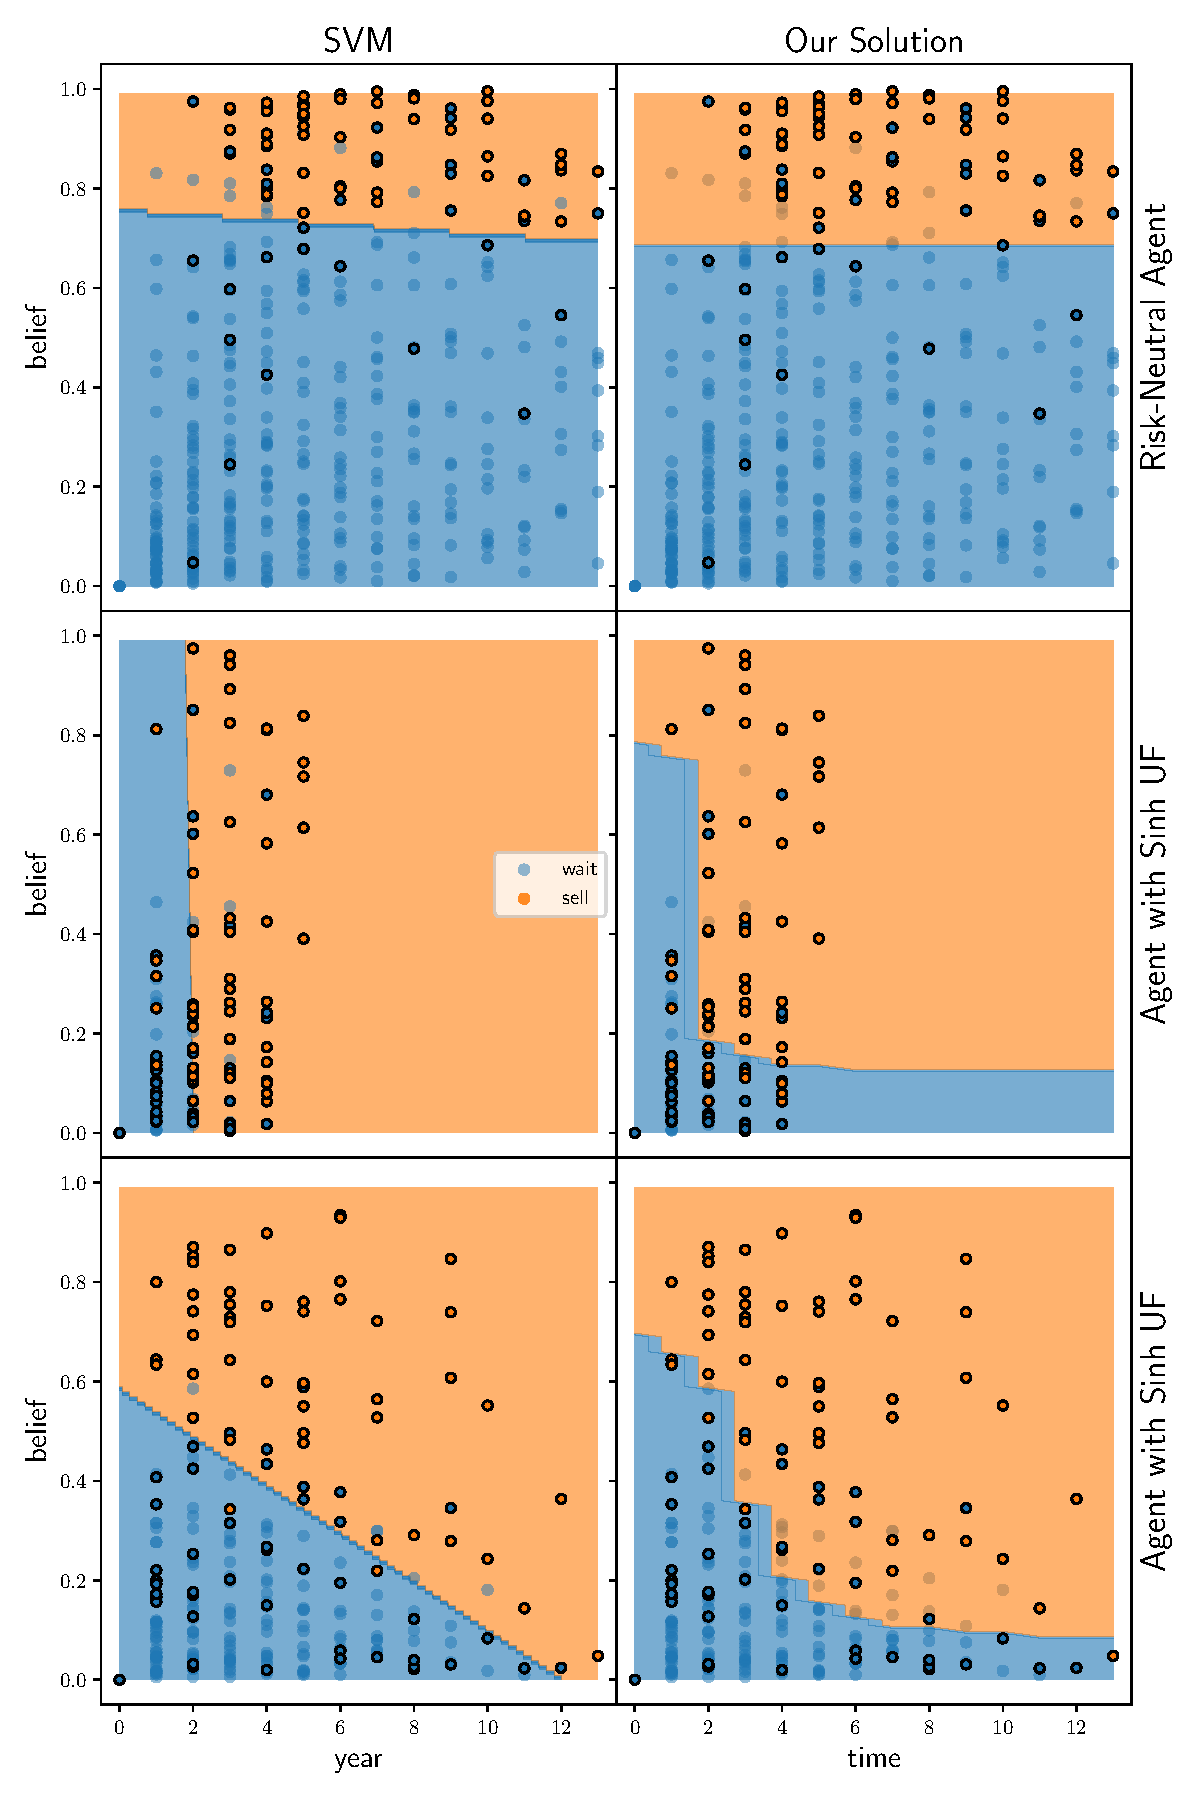
\includegraphics[width=0.99\linewidth]{img/fit}
    \caption{Examples from three human behaviors distinctly observed and reproduced with RL agents. Behaviors by row: 1) Constant belief threshold, modeled by the risk-averse exponential utility function, 2) Fixed time threshold, modeled by sinh utility, 3) Mixed strategy, modeled by sinh exponential utility. The left column shows the empirical optimal split of data using linear kernel support vector machine (with cross-validation). The right column shows optimal policy that is closest to the SVM split, found via grid-search.}
    \label{fig:svm_vs_value}
\end{figure}

\subsection{From human behavior to utility functions}\label{ssec:human-behavior}

In~\autoref{ssec:val-func}, we have presented how different utility functions result in different policies.
Now we look at how we derived utility functions and the corresponding risk parameters from behavioral data.
In literature, this is called \keyword{inverse reinforcement learning} \cite{Abbeel2010}.

Inverse reinforcement learning is challenging. Thus, we only try a naive approach, which can be summarized in three steps: 1) observe behavior, 2) estimate policy, and 3) derive utility functions and risk parameters using a grid-search.
The results are plotted in~\autoref{fig:svm_vs_value}, and explained in following. 
First, we get behavioral data for a subject from the expert-setting of the experiment.
For each time step (i.e. year) of each trial, we have a data point with the action subject took, the belief shown to the user and the year. These are plotted in~\autoref{fig:svm_vs_value} with blue for wait action, and orange for sell action.

Second, we estimate the policy using a SVM \cite{svm} with cross-validation. SVM tries to fit a decision boundary, which minimizes the wait actions above and sell actions below this boundary. Here we only take the last two actions into account, i.e. one waiting and one selling actions (plotted with fuller circles), the rest of the actions are plotted in light colors.

The last step is to perform a grid search over the utility functions and their parameters.
Each utility function and its parameters results in a value function from which a policy is derived.
The goal of the grid search is to find the policy that is closest to the SVM decision boundary.

We found $\text{sinh}$ and Exponential UF to work the best. In behavioral data, we observed three kinds of behaviors: 1) people selling at a specific belief threshold, 2) people selling at a specific year, and 3) people lowering their threshold over years. We show an example for each of these behaviors in each row of~\autoref{fig:svm_vs_value}.



\subsection{Analysis of agents}
After reproducing the human behavior with agents, we can compare the performance of different agents.
We sampled 10.000 episodes with each agent and present their performance in~\autoref{fig:perf}. The accumulated reward of each agent is presented with a box plot, where the green line shows the median of the accumulated reward, the box shows the Q1-Q3 quartile, and the circles show the outliers\footnote{Refer to matplotlib documentation and Wikipedia for an exact description of a box plot: \url{https://matplotlib.org/api/_as_gen/matplotlib.pyplot.boxplot.html}, \url{https://en.wikipedia.org/wiki/Quartile}}.
The ratio of sells in the good state is shown with a bar plot.
Here, bars show the ratio of selling in the good state and the black lines show the variance.

The risk-averse agent has lower variance both on average reward, and the ratio of selling in the good state. However, it has a similar number of outliers in accumulated reward as the risk-neutral agent, which can be easily explained by the high selling threshold that results in a longer waiting time. The agents using sinh UF, on the other hand, have no outliers. And the mixed strategy has a similar median value with slightly larger quartile.
This shows the benefit of risk modeling, even in such simple scenarios.

\begin{figure}[h]
    \centering
    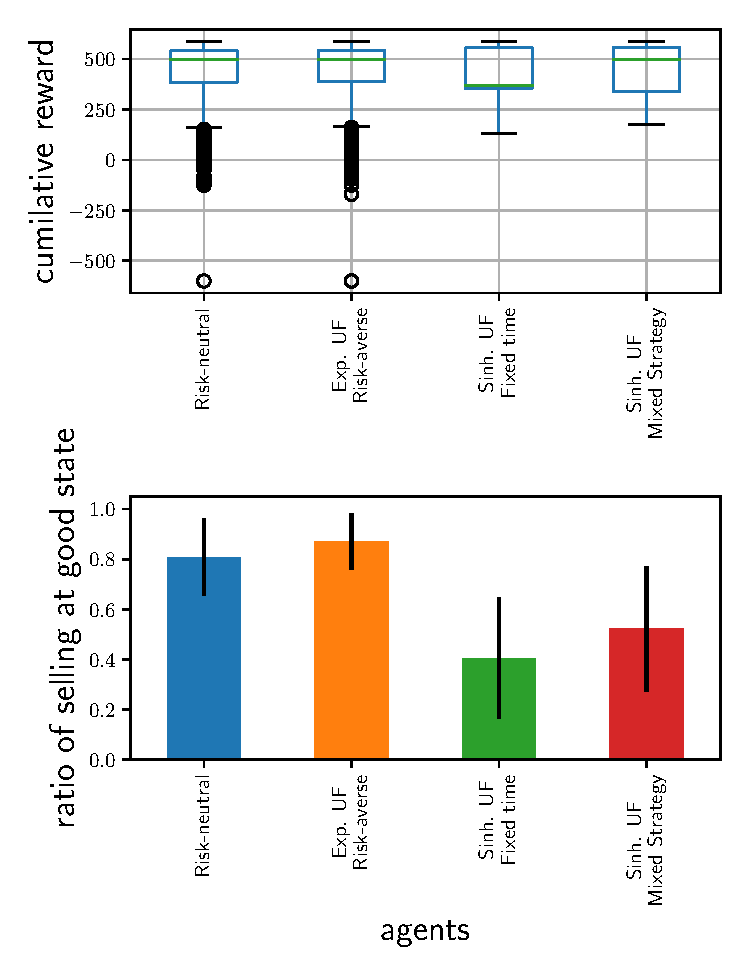
\includegraphics[width=0.99\linewidth]{img/performance.pdf}
    \caption{Accumulated reward and ratio of selling in the good state.}\label{fig:perf}
\end{figure}
